\setbeamertemplate{headline}[backup]
\setbeamertemplate{footline}[backup]





    %%%%%%%%%%%%%%%%%%%%%%%%%%%%%%%%%%%%%%%%
    %%  Slide 1: <BACKUP>  %%
    %%%%%%%%%%%%%%%%%%%%%%%%%%%%%%%%%%%%%%%%
    \begin{frame}[noframenumbering]
        Backup        
    \end{frame} 

    %%%%%%%%%%%%%%%%%%%%%%%%%%%%%%%%%%%%%%%%
    %%  Slide 3: <Sensors types>  %%
    %%%%%%%%%%%%%%%%%%%%%%%%%%%%%%%%%%%%%%%%
    \begin{frame}[noframenumbering]
        \frametitle{MAPS sensor types}
            \begin{itemize}
                \item \textbf{Large fill factor} ($\sim$100-200 \si{fF}) or \textbf{small fill factor} ($<$\SI{5}{fF}), depending on the deep p-well structures
            \end{itemize}
            %\centering
            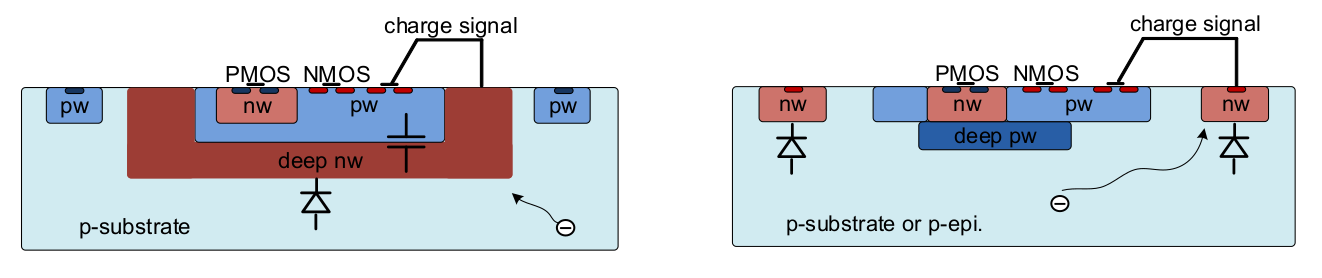
\includegraphics[width=1.05\linewidth]{figures/Pixel_detectors/large_small_sensor_scheme.png}\\
            \begin{columns}
                \column{0.5\textwidth}  
                    %\centering
                    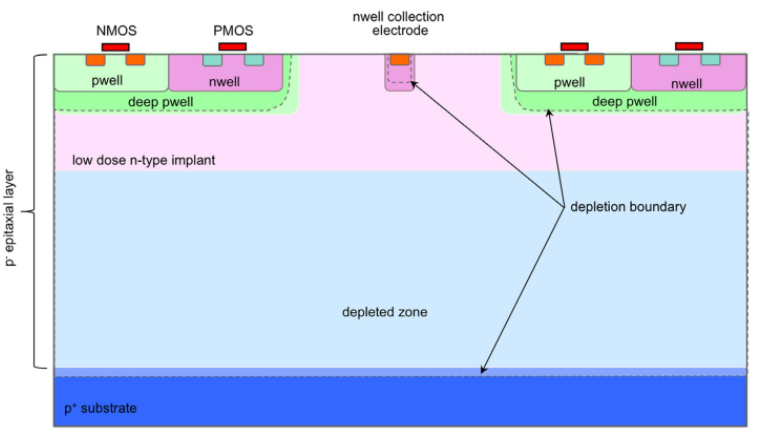
\includegraphics[width=1.1\linewidth]{figures/Pixel_detectors/ALPIDE_after_PM.png}
                \column{0.5\textwidth}  
                    \begin{itemize}
                        \item \textbf{Process modification} with a low dose planar implant. \\
                        whose main investigator is ALICE\\
                        %Advantage: no need of change in the sensor and circuit layout
                    \end{itemize} 
            \end{columns}

            \end{frame} 

    %%%%%%%%%%%%%%%%%%%%%%%%%%%%%%%%%%%%%%%%
    %%  Slide 1: <Applications>  %%
    %%%%%%%%%%%%%%%%%%%%%%%%%%%%%%%%%%%%%%%%
    %\begin{frame}
    %    \frametitle{Tracking in HEP}

    %    Task of pixel detectors in tracking:
    %    \begin{itemize}
    %        \item pattern recognition with the identification of particle tracks even in the presence of large backgrounds and pile-up
    %        \item measurement of vertices (primary and secondary)
    %        \item multi-track and vertex separation in the core of jets
    %        \item measurement of specific ionization
    %        \item momentum measurement combining with the information from other detectors
    %    \end{itemize}
    %\end{frame} 

    %%%%%%%%%%%%%%%%%%%%%%%%%%%%%%%%%%%%%%%%
    %%  Slide 1: <ALICE>  %%
    %%%%%%%%%%%%%%%%%%%%%%%%%%%%%%%%%%%%%%%%
    \begin{frame}[noframenumbering]
        \frametitle{Belle2 vertex detector}
        Thin detector needed for a precise reconstruction of B-decay vertices
        \begin{columns}
            \column{0.4\textwidth}  
                \textbf{VXD} made by:
                \begin{itemize}
                    \small
                    \item PXD $\rightarrow$ 2 DEPFET layers
                    \item SVD $\rightarrow$ 4 strip layers
                \end{itemize}
            \column{0.6\textwidth}
                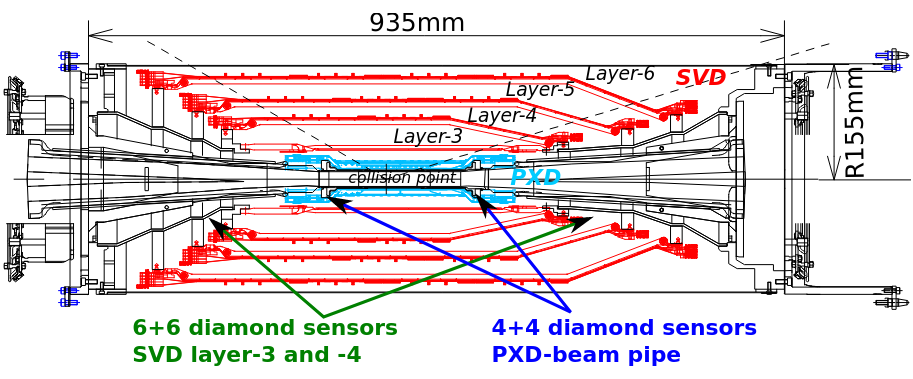
\includegraphics[width=1.1\linewidth]{figures/pixel_detectors_usage/SVD_Belle2.png}
        \end{columns}
        Replacement of VXD with \textbf{VTX}, proposed for LSH2. VTX should be made of 5 layers of CMOS MAPS
        \begin{itemize}
            \item improvements in the track and vertex resolutions
            \item reduction in the material budget
            \item higher background tolerance because
            of the smaller sensor (pixels than strips)
        \end{itemize}
    \end{frame} 



    %%%%%%%%%%%%%%%%%%%%%%%%%%%%%%%%%%%%%%%%
    %%  Slide 1: <ALICE>  %%
    %%%%%%%%%%%%%%%%%%%%%%%%%%%%%%%%%%%%%%%%
    \begin{frame}[noframenumbering]
        \frametitle{ALPIDE - ALice PIxel DEtector}
        ALICE ITS2 upgraded in 2019-20\\
        \smallskip
        The \textbf{sensor} uses high resistivity p-type epi-layer, TowerJazz in \SI{0.18}{\um}. It is the first large area $\sim$\SI{10}{m\squared} MAPS detector with sparsified readout.
        Many MAPS have an \textbf{ALPIDE-based Front End} (i.e. TJ-Monopix1, ARCADIA)
        \begin{columns}
            \column{0.35\textwidth}  
                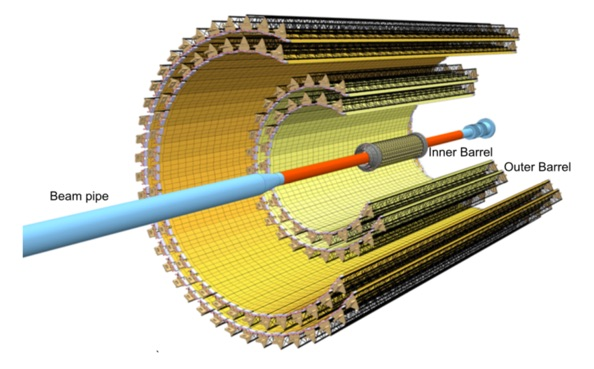
\includegraphics[width=1.3\linewidth]{figures/pixel_detectors_usage/alice.png}
            \column{0.6\textwidth}
            \begin{itemize}
                \item position resolution $\sim$\SI{5}{\um} (pixel dimension 27$\times$29\si{\um\squared})
                \item X$_0$/layer reduced from 1.14\% to 0.3\%
                \item tracking efficiency of low-p$_T$ ($p_T \sim$\SI{0.1}{GeV/c}) improved by a factor 6
            \end{itemize}
        \end{columns}
        %ALPIDE is under test for several other HEP detectors (i.e. Belle2) and applications and 
    \end{frame} 

     %%%%%%%%%%%%%%%%%%%%%%%%%%%%%%%%%%%%%%%%
    %%  Slide 1: <>  %%
    %%%%%%%%%%%%%%%%%%%%%%%%%%%%%%%%%%%%%%%%
    \begin{frame}[noframenumbering]
        \frametitle{ALPIDE front end}
            \textbf{ALPIDE like}: circuit implemented in TJ-Monopix1
            \begin{figure}[h!]
                \centering
                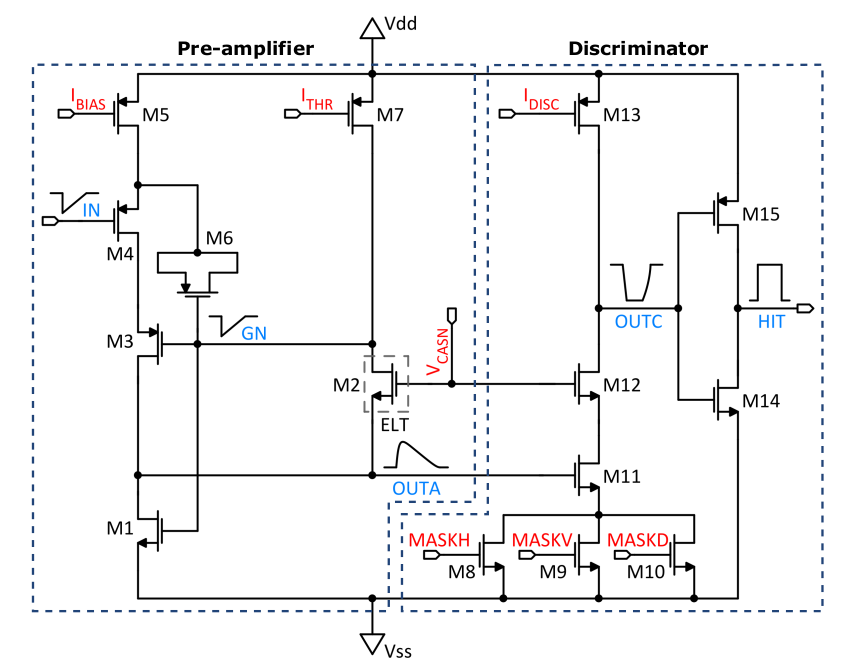
\includegraphics[width=.8\linewidth]{figures/Monopix1/Monopix1_FE_circuit.png}        
            \end{figure}
    \end{frame}     

        %%%%%%%%%%%%%%%%%%%%%%%%%%%%%%%%%%%%%%%%
    %%  Slide 1: <>  %%
    %%%%%%%%%%%%%%%%%%%%%%%%%%%%%%%%%%%%%%%%
    \begin{frame}[noframenumbering]
        \frametitle{TJ-Monopix1 readout sequence}
        \begin{columns}
            \column{0.6\textwidth}             
            \centering
            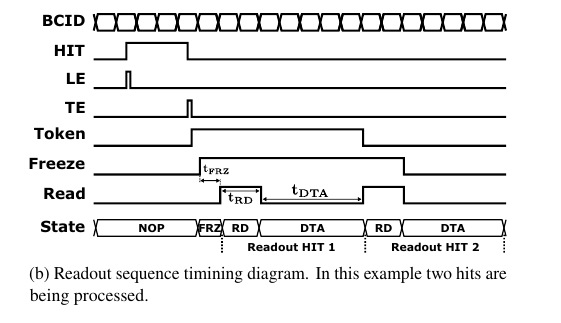
\includegraphics[width=1.\linewidth]{figures/Monopix1/readout_timing.png}
        \column{0.4\textwidth}    
        \textbf{BCID} = Bunch Crossing identification
        is the clock of the timestamp   \\
        \end{columns}
        \begin{itemize}
            \item The \textbf{token} manage the priority chain
            \item The \textbf{freeze} is a global signal and is used to lock the matrix during the readout. \\
            \small Pixels without any hit can store new data but they cannot access the priority chain untill the freeze stops
            \item The \textbf{read} is used to indicate when the pixel can access the data bus
        \end{itemize}
    \end{frame} 


    %%%%%%%%%%%%%%%%%%%%%%%%%%%%%%%%%%%%%%%%
    %%  Slide 1: <>  %%
    %%%%%%%%%%%%%%%%%%%%%%%%%%%%%%%%%%%%%%%%
    \begin{frame}[noframenumbering]
        \frametitle{TJ-Monopix1: noisy pixels}
        The masking algorithm uses 3 cordinates to mask a pixel: 
        \begin{columns}
            \column{0.55\textwidth} 
            \small
            \begin{itemize}
                \item MASKV $\rightarrow$ column of the pixel
                \item MASKH $\rightarrow$ row of the pixel
                \item MASKD $\rightarrow$ diagonal of the pixel
            \end{itemize}   
            \centering             
            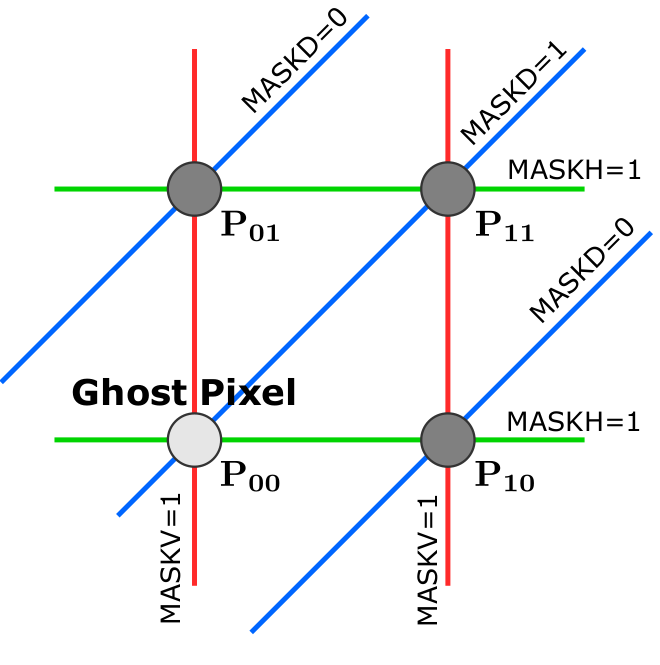
\includegraphics[width=.7\linewidth]{figures/Monopix1/masking_scheme.png}        
                \column{0.5\textwidth} 
                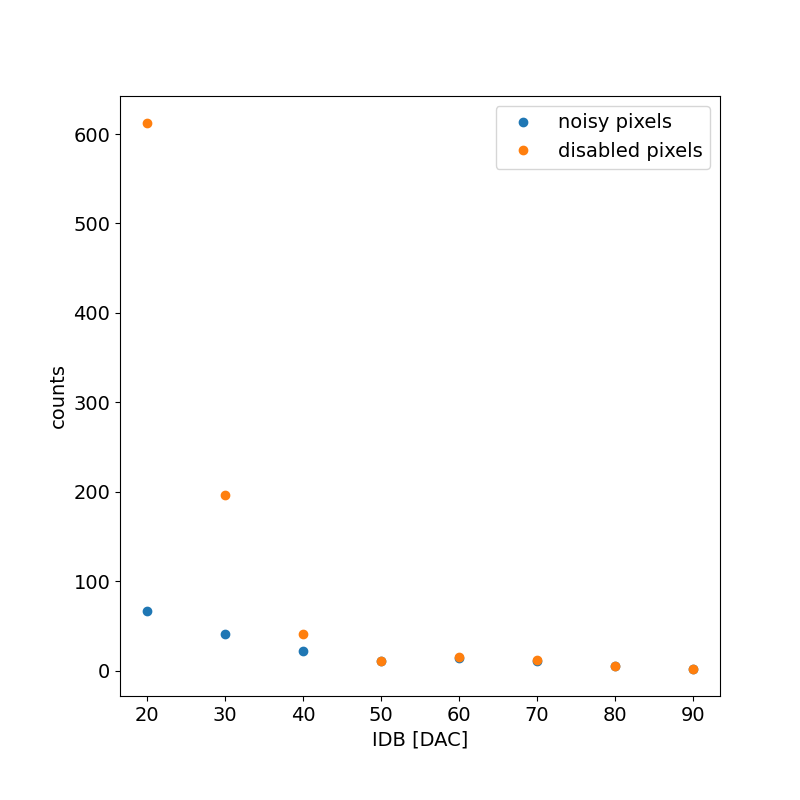
\includegraphics[width=1.1\linewidth]{figures/charaterization/noisy.png}
                \centering IDB = discriminator threshold 
        \end{columns}

    \end{frame}   

    %%%%%%%%%%%%%%%%%%%%%%%%%%%%%%%%%%%%%%%%
    %%  Slide 4: <ToT calibration>  %%
    %%%%%%%%%%%%%%%%%%%%%%%%%%%%%%%%%%%%%%%%
    \begin{frame}[noframenumbering]
        \frametitle{Different collection properties}
        2 different \textbf{dose profile} in the sensor: Reduced Deep P-Well (RDPW) and Full Deep P-Well (FDPW) with different charge collection efficiency
        \begin{columns}
            \column{0.5\textwidth}                  
                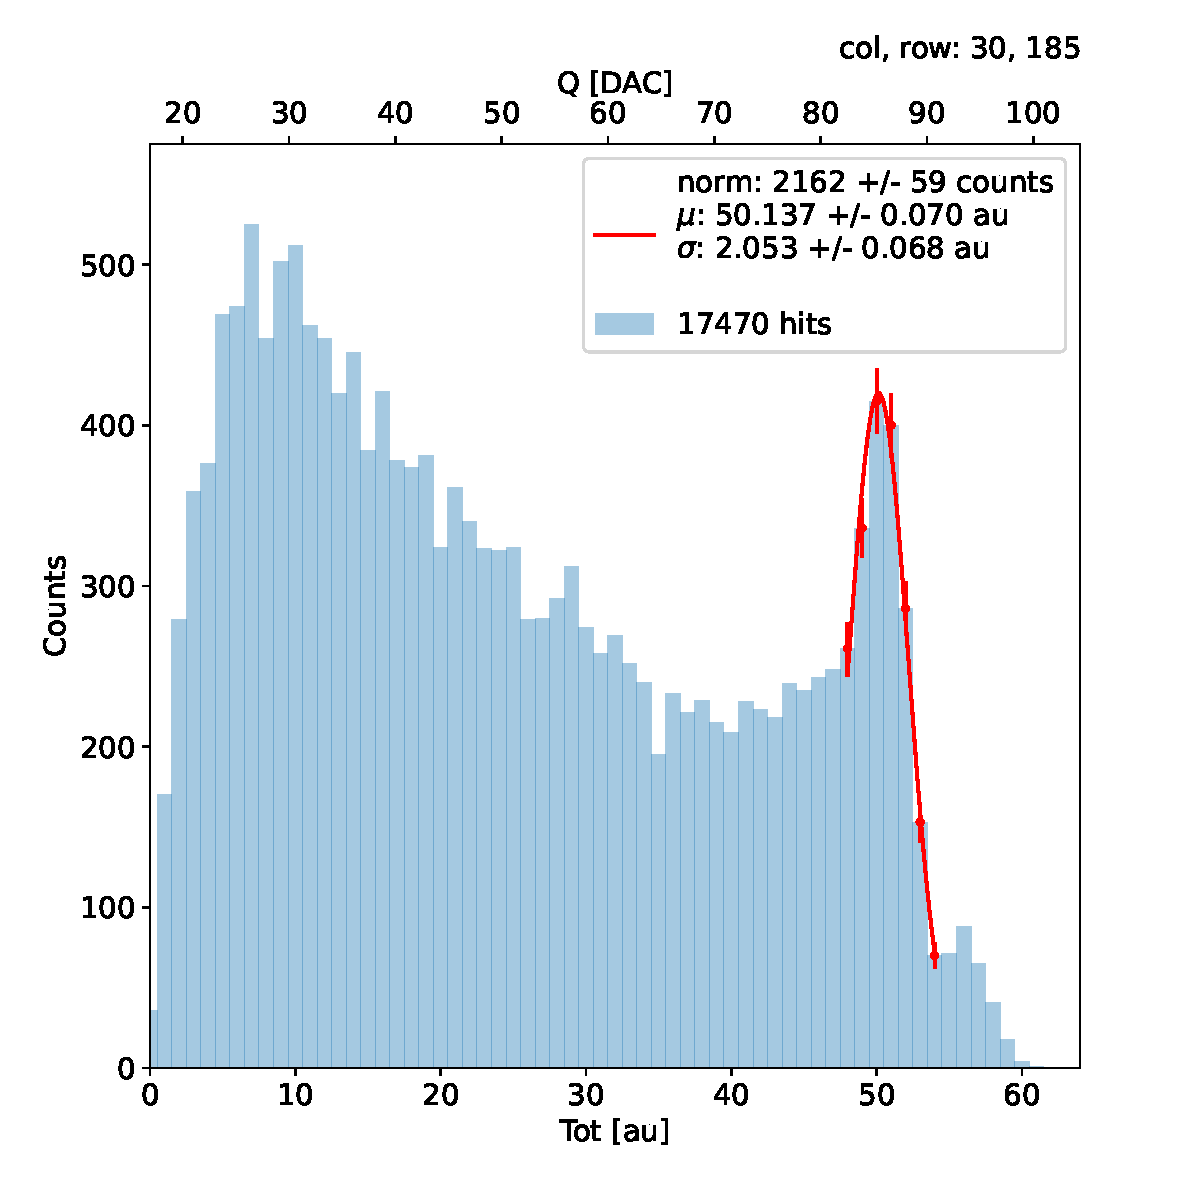
\includegraphics[width=1.\linewidth]{figures/charaterization/fit_gauss_r185.pdf}
                \centering Partial deep p-well
            \column{0.5\textwidth}    
                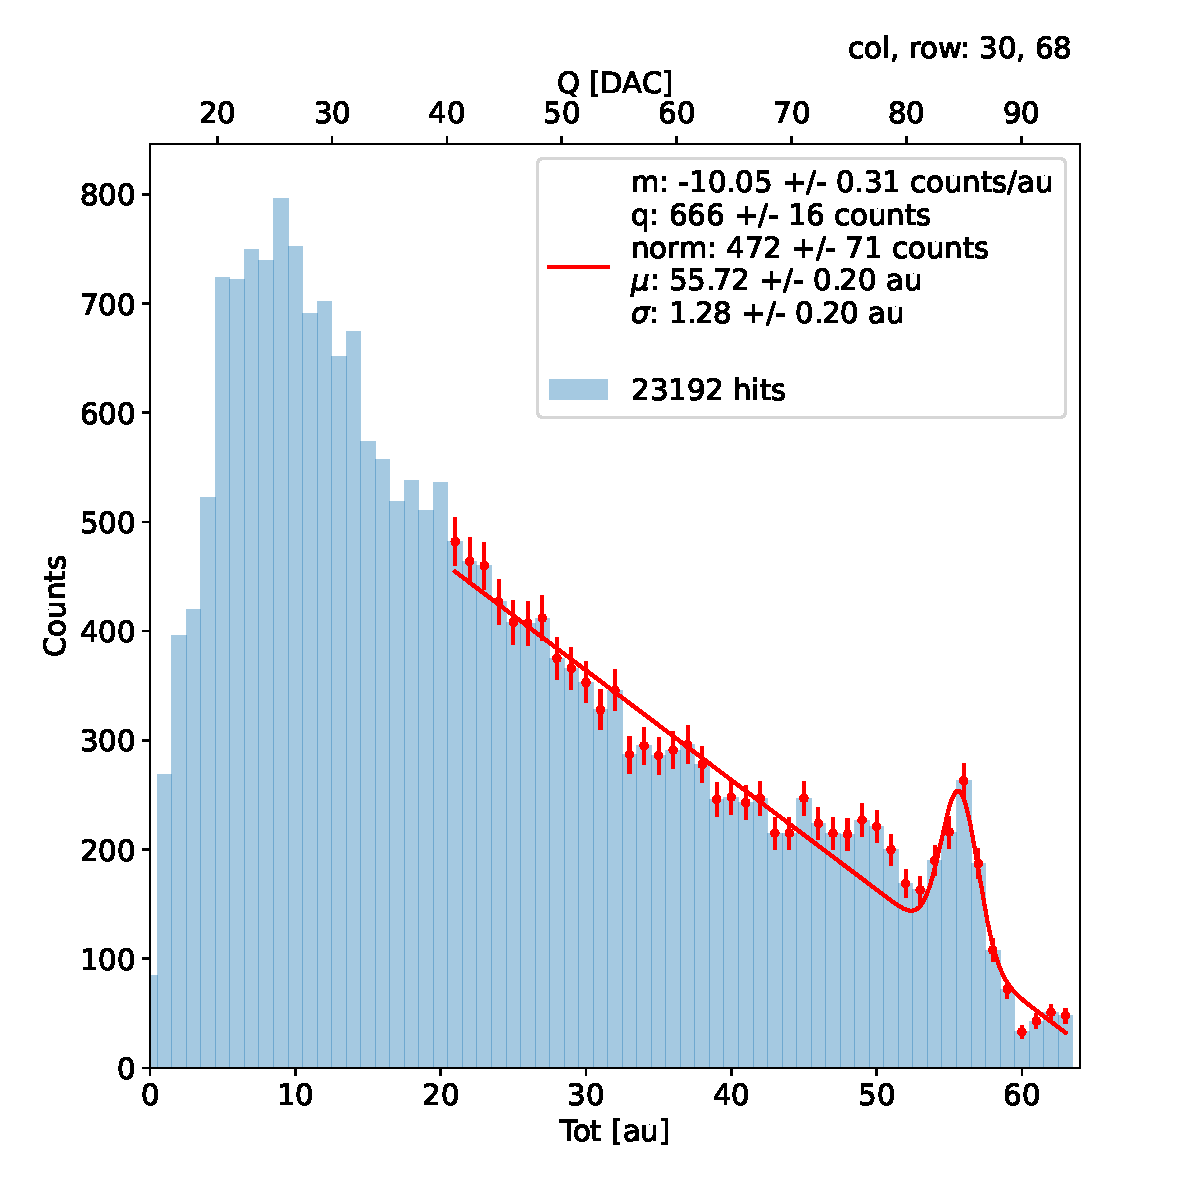
\includegraphics[width=1.\linewidth]{figures/charaterization/fit_line_gauss_r69.pdf}
                \centering Full deep p-well
        \end{columns}
    \end{frame}





    \begin{frame}[noframenumbering]
        \frametitle{Threshold and noise results with different FEs}
        \begin{columns}
            \column{0.45\textwidth}        
                \includegraphics[width=.95\linewidth]{figures/charaterization/threshold_allflavors_presentazione.pdf}
            \column{0.45\textwidth}        
                \includegraphics[width=.95\linewidth]{figures/charaterization/noise_allflavors_presentazione.pdf} 
        \end{columns}                  
        %\hspace*{+0.1cm}
        \begin{table}[h!]
            \footnotesize
            \begin{tabular}{| c |  c | c | c |c || c|}
            \hline
            & PMOS A & PMOS B & PMOS C & HV & simulation \\
            \hline
            \hline
            $\mu$ [\si{\elementarycharge}$^-$] & 401.7$\pm$0.2 & 400.8$\pm$0.2 & 539.7$\pm$0.6 &  597.7$\pm$0.3 & $\sim$270\\
            $\Delta_{\mu}$ [\si{\elementarycharge}$^-$] & 32.9$\pm$0.1 & 33.0$\pm$0.2 & 55.5$\pm$0.4 & 66.1$\pm$0.3 & $\sim$30\\
            $\sigma$ [\si{\elementarycharge}$^-$] & 13.01$\pm$0.06 & 12.26$\pm$0.07 & 13.9$\pm$0.1 & 17.3$\pm$0.1 & $\sim$9 \\
            $\Delta_{\sigma}$ [\si{\elementarycharge}$^-$] & 1.61$\pm$0.04 & 1.50$\pm$0.05 & 1.91$\pm$0.07 & 2.3$\pm$0.1 & -\\
            \hline
            \end{tabular}
        \end{table}       
    \end{frame}




    %%%%%%%%%%%%%%%%%%%%%%%%%%%%%%%%%%%%%%%%
    %%  Slide 4: <Aquisitions with sources>  %%
    %%%%%%%%%%%%%%%%%%%%%%%%%%%%%%%%%%%%%%%%
    \begin{frame}[noframenumbering]
        \frametitle{Acquisition with sources: Fe$^{55}$, Sr$^{90}$, cosmic rays}
        \begin{columns}
            \column{0.6\textwidth} 
                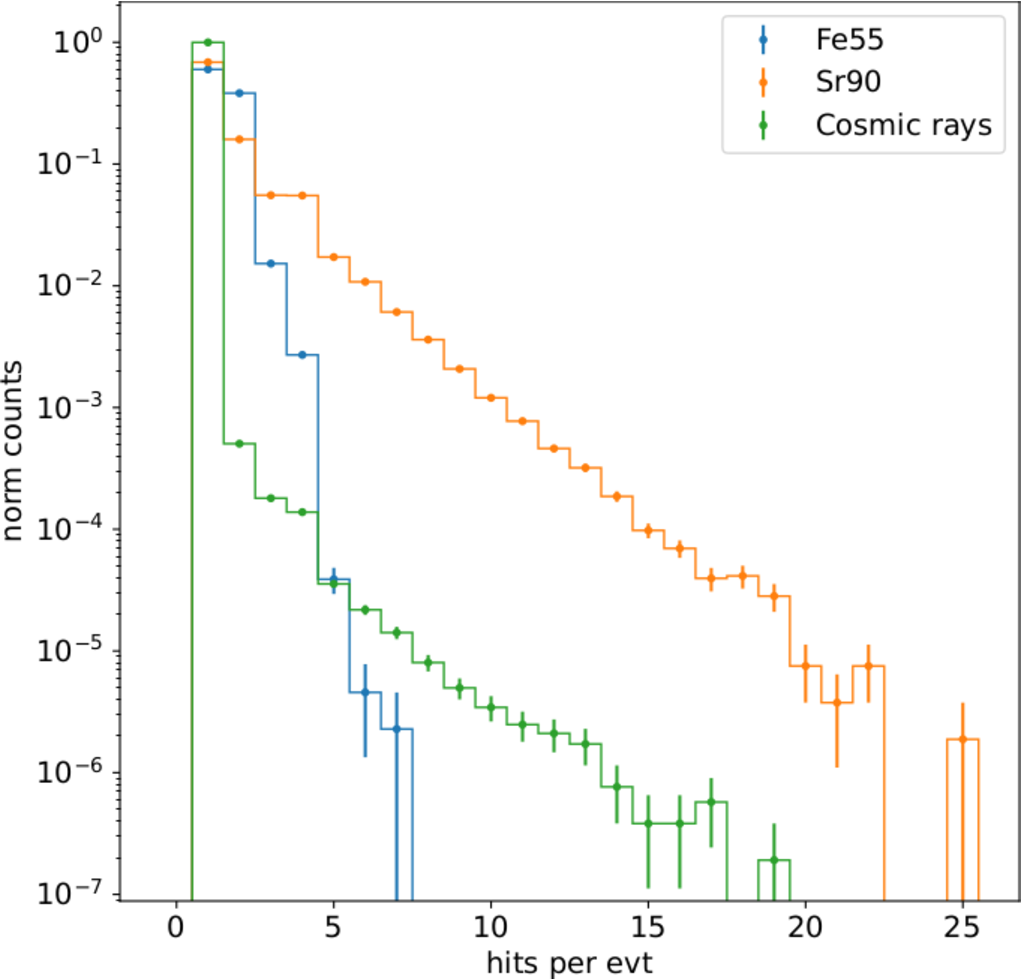
\includegraphics[width=1.\linewidth]{figures/charaterization/hits_per_evt.png}
            \column{0.4\textwidth} 
                \begin{itemize}
                    \item Fe$^{55}$ photon produces smaller clusters: pure charge sharing
                    \item Sr$^{90}$ and cosmic rays go across more pixels 
                \end{itemize}    
        \end{columns}
    \end{frame}    

 




    %%%%%%%%%%%%%%%%%%%%%%%%%%%%%%%%%%%%%%%%
    %%  Slide 1: <>  %%
    %%%%%%%%%%%%%%%%%%%%%%%%%%%%%%%%%%%%%%%%
    \begin{frame}[noframenumbering]
        \frametitle{Radiotherapy}
        \begin{columns}
            \column{0.4\textwidth}  
            Many different sources: 
            \begin{itemize}
                \item hadrons $\rightarrow$ Bragg peak 
                \item photons $\rightarrow$ exponential absoption
                \item electrons $\rightarrow$ $\sim$\SI{10}{MeV} or VHEE $\sim$\SI{100}{MeV}
            \end{itemize}
            \column{0.6\textwidth}  
                \begin{figure}[h!]
                    \centering
                    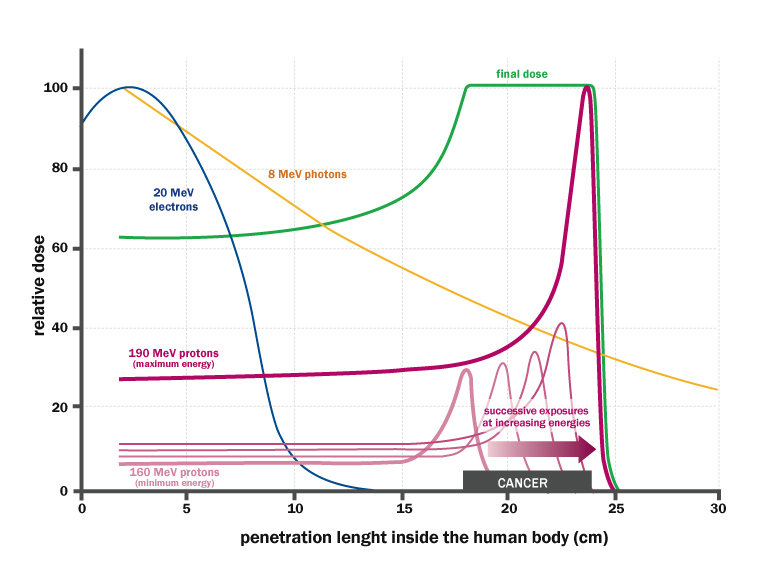
\includegraphics[width=1.\linewidth]{figures/pixel_detectors_usage/Bragg-Peak.png}
                \end{figure}
        \end{columns}
    \end{frame} 

    %%%%%%%%%%%%%%%%%%%%%%%%%%%%%%%%%%%%
    %% Slide 2: <> %%
    %%%%%%%%%%%%%%%%%%%%%%%%%%%%%%%%%%%%
    \begin{frame}[noframenumbering]
        \frametitle{Test on the beam: ElectronFLASH}
        ElectronFLASH is the new accelerator for research on FLASH-RT placed in S. Chiara hospital in Pisa \\
        \medskip
        Accelerator charateristics: 
        \begin{itemize}
            \item linear accelerator
            \item bunched beam
            \item two energy configurations 7-9\si{MeV}
            \item can reach ultra high intensity (over \SI{5000}{Gy/s})
            \item beam parameters can be configured independently from each other
            \item equipped with a set of plexiglass applicators (diameters in range from \SI{1}{cm} to \SI{12}{cm}) which are used to produce a uniform dose profile 
        \end{itemize}
    \end{frame}  

    %%%%%%%%%%%%%%%%%%%%%%%%%%%%%%%%%%%%
    %% Slide 3: <> %%
    %%%%%%%%%%%%%%%%%%%%%%%%%%%%%%%%%%%%
    \begin{frame}[noframenumbering]
        \frametitle{Test on beam: preliminary results}
        \begin{itemize}
            \item With \textbf{both} the collimators, DPP=\SI{0.07}{Gy}, t$_p$=\SI{4}{\us}, PRF=\SI{1}{Hz}
        \end{itemize}
        \medskip
        \begin{figure}
            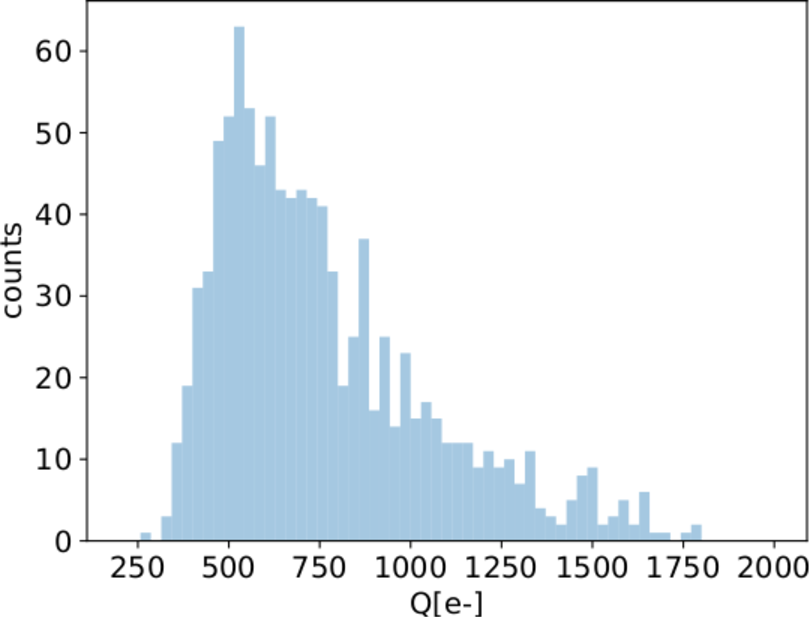
\includegraphics[width=0.49\linewidth]{figures/test_beam/Q1_17_11.pdf}
            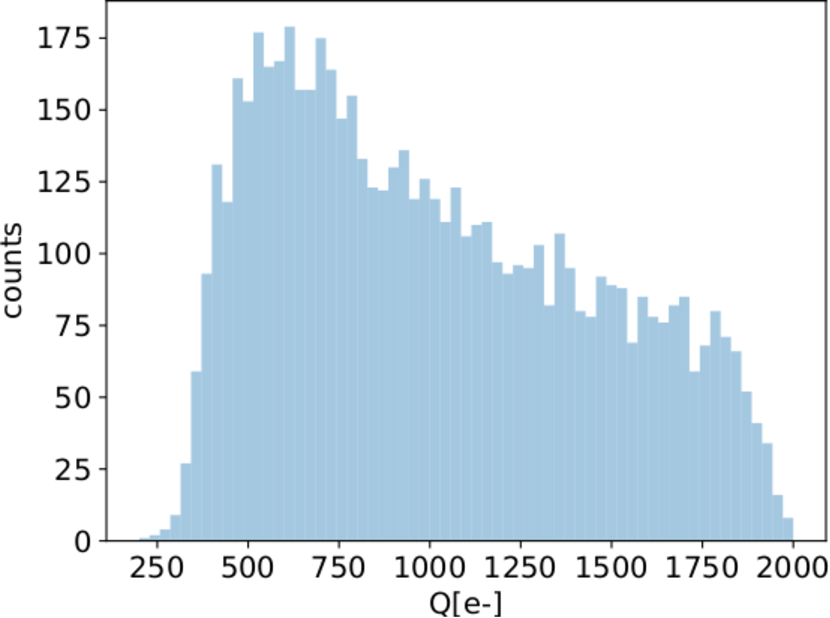
\includegraphics[width=.49\linewidth]{figures/test_beam/Q2_17_11.pdf}
        \end{figure}
        \begin{itemize}
            \item the collimators do not shield the detectors from all particles
            \item probably photons are produced by electrons in Al collimators
            \item for each accelerator pulse, 2 readout "cycle"  
        \end{itemize}
    \end{frame} 
    
    %%%%%%%%%%%%%%%%%%%%%%%%%%%%%%%%%%%%
    % Slide 3: <> %%
    %%%%%%%%%%%%%%%%%%%%%%%%%%%%%%%%%%%%
    \begin{frame}[noframenumbering]
        \frametitle{Test on beam: preliminary results}
        \begin{itemize}
            \item\textbf{Without} any collimator, DPP=\SI{0.04}{Gy}, t$_p$=\SI{4}{\us}, PRF=\SI{1}{Hz}
            \item MIP are expected to release \SI{2000}{\elementarycharge}$^-$, and because of rollorver are expected to be 300-400\si{\elementarycharge}$^-$
        \end{itemize}
        \medskip
        \begin{columns}
            \column{0.5\textwidth} 
                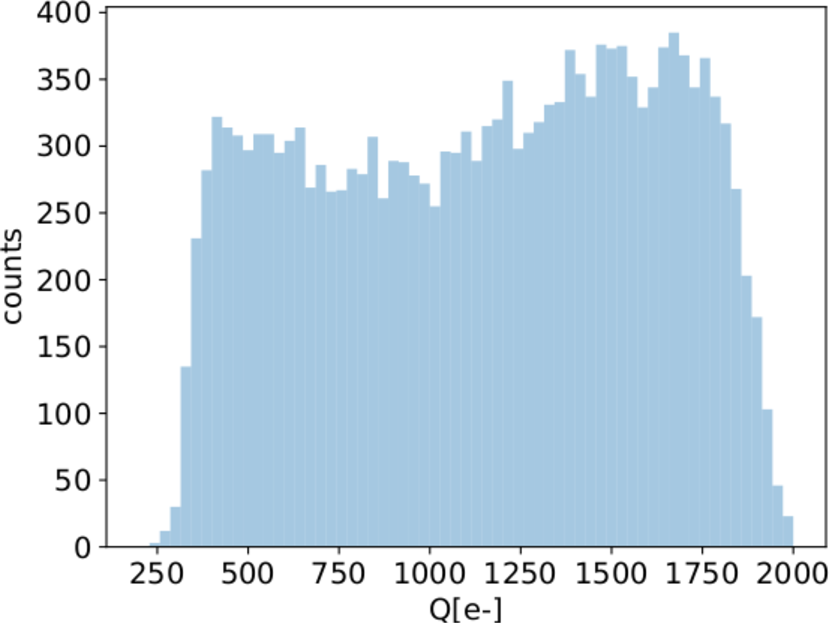
\includegraphics[width=1.1\linewidth]{figures/test_beam/Qe_17_32.pdf}
            \column{0.5\textwidth} 
                \begin{itemize}
                    \item ToT converted in charge
                    \item pixels turn on in N clock counts
                    \item after each pulse an induced signal on the whole matrix
                \end{itemize}
        \end{columns}   
        \medskip
        Need for a simulation to understand the data
    \end{frame}   





    %%%%%%%%%%%%%%%%%%%%%%%%%%%%%%%%%%%%
    %% Slide 2: <> %%
    %%%%%%%%%%%%%%%%%%%%%%%%%%%%%%%%%%%%
    \begin{frame}[noframenumbering]
        \frametitle{ARCADIA MD1}
        \begin{columns}
            \column{0.5\textwidth}        
                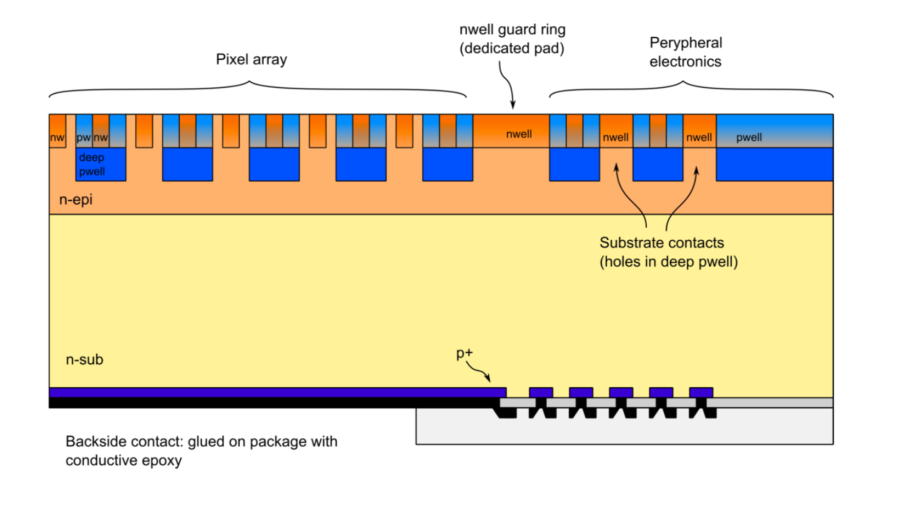
\includegraphics[width=1.05\linewidth]{figures/ARCADIA/sensor.png}
                \begin{itemize}
                    \item produced by LFoundry (Italy)
                    \item 110 nm CMOS technology
                    \item n-doped epitaxial layer
                \end{itemize}
            \column{0.5\textwidth}        
                \begin{table}[h!]
                    \footnotesize
                    \begin{tabular}{| c |c |}
                    \hline
                    Parameter & Value\\
                    \hline
                    \hline
                    Matrix size & 1.28$\times$1.28 \si{cm\squared}\\
                    Number of pixels & 512$\times$512\\
                    Pixel size & 25$\times$25 \si{\um\squared}\\
                    Depth &  48/100/200\si{\um}\\
                    Electrode size & 9$\times$9\si{\um\squared}\\
                    Power consumption & $\sim$ 10\si{mW/cm\squared}\\ 
                    Output signal & digital \\
                    \hline
                    \end{tabular}
                \end{table}
        \end{columns}                  
    \end{frame}




    %%%%%%%%%%%%%%%%%%%%%%%%%%%%%%%%%%%%
    %% Slide 2: <> %%
    %%%%%%%%%%%%%%%%%%%%%%%%%%%%%%%%%%%%
    \begin{frame}[noframenumbering]
        \frametitle{ARCADIA MD1: experimental setup}
            \includegraphics[width=.95\linewidth]{figures/ARCADIA/setup_foto.pdf}
    \end{frame}


    %%%%%%%%%%%%%%%%%%%%%%%%%%%%%%%%%%%%
    %% Slide 2: <> %%
    %%%%%%%%%%%%%%%%%%%%%%%%%%%%%%%%%%%%
    \begin{frame}[noframenumbering]
        \frametitle{ARCADIA MD1: matrix division}
            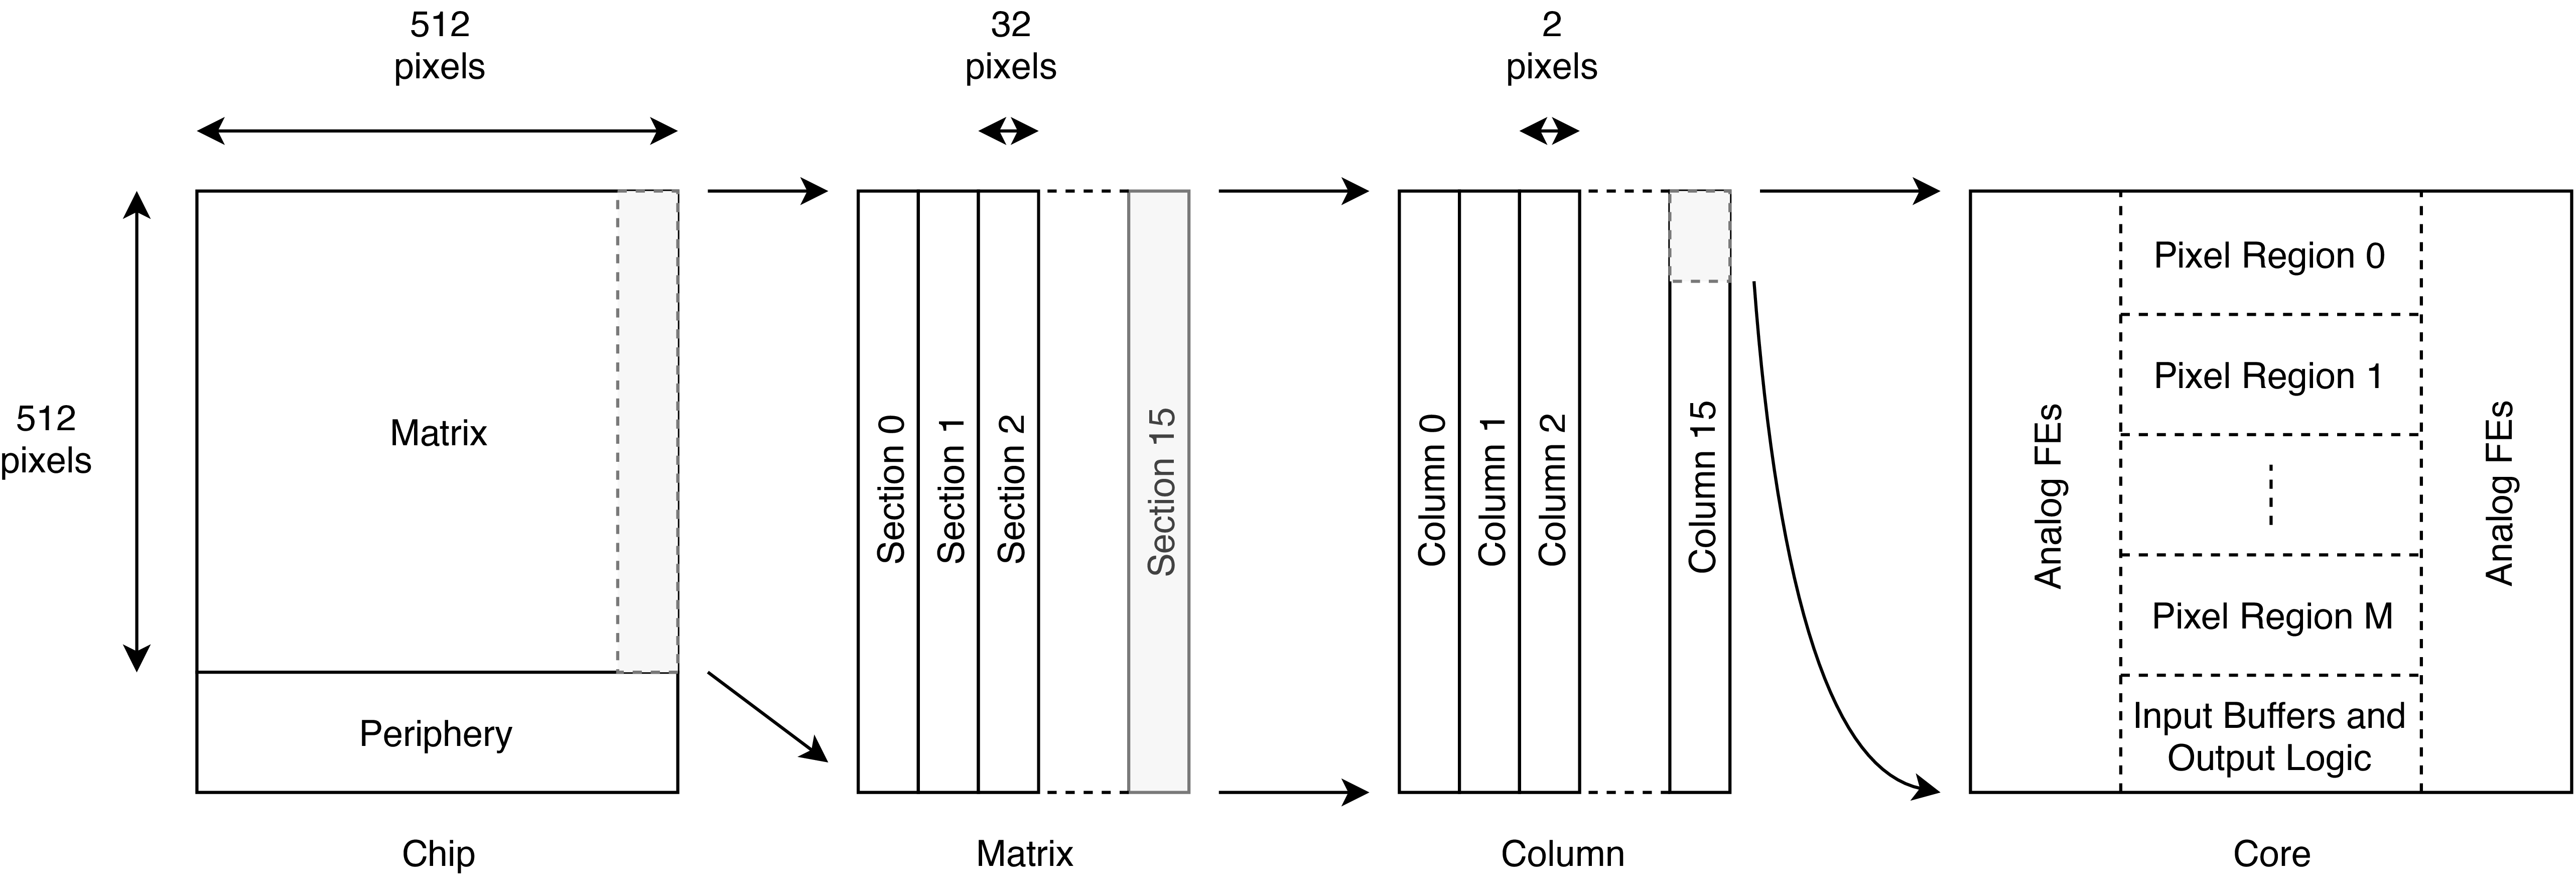
\includegraphics[width=1.\linewidth]{figures/ARCADIA/hierarchy.png}
            \begin{columns}
                \column{0.65\textwidth}   
                    The matrix contains 512$\times$512 pixels divided in:
                    \begin{itemize}
                        \item 16 sections containing 512$\times$32 pixels
                        \item 512$\times$2 double columns
                        \item cores of 32$\times$2 pixels
                        \item regions contaning 4$\times$2 pixels $\rightarrow$ regions can be master or slave
                    \end{itemize}
                \column{0.35\textwidth}   
                    \begin{table}
                        \begin{tabular}{|c |c |}
                        \hline
                        Bits & Meaning  \\
                        \hline
                        \hline
                        31:24 & timestamp\\
                        23:20 & section index\\
                        19:16 & column index\\
                        15:9 & pixel region\\
                        8:0 & hitmap\\
                        \hline
                        \end{tabular}
                    \end{table}
            \end{columns}
    \end{frame}

        %%%%%%%%%%%%%%%%%%%%%%%%%%%%%%%%%%%%
    %% Slide 2: <> %%
    %%%%%%%%%%%%%%%%%%%%%%%%%%%%%%%%%%%%
    \begin{frame}[noframenumbering]
        \frametitle{ARCADIA MD1: clustering}
            \textbf{Clustering} allows trasmit less data packet, 
            \textit{Master} regions can decide what \textit{slaves} data to trasmit
            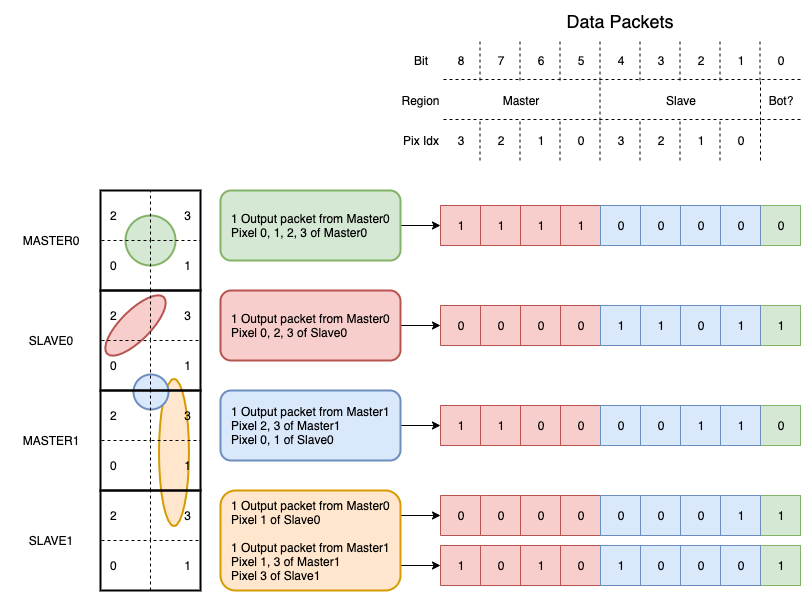
\includegraphics[width=.85\linewidth]{figures/ARCADIA/clustering.png}
    \end{frame}

    %%%%%%%%%%%%%%%%%%%%%%%%%%%%%%%%%%%%
    %% Slide 2: <> %%
    %%%%%%%%%%%%%%%%%%%%%%%%%%%%%%%%%%%%
    \begin{frame}[noframenumbering]
        \frametitle{ARCADIA MD1: clustering}
            %Without clustering
            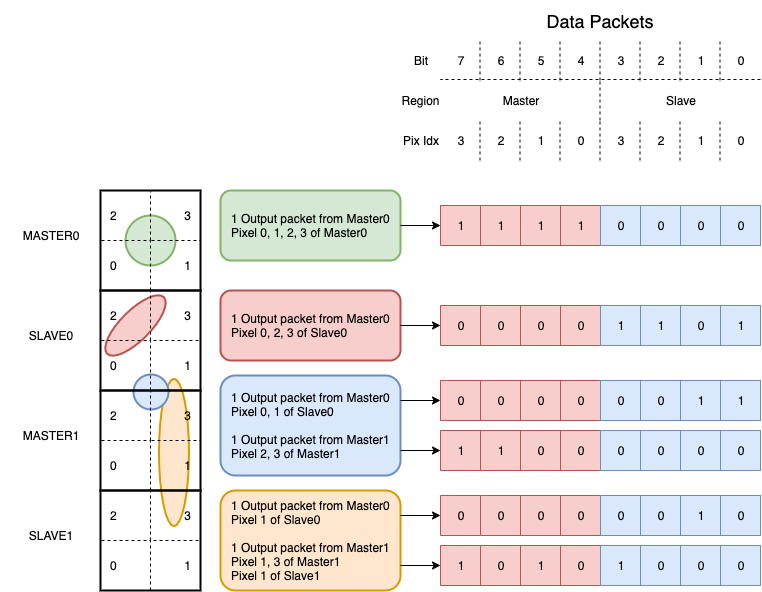
\includegraphics[width=.9\linewidth]{figures/ARCADIA/nonclustering.png}
    \end{frame}



    %%%%%%%%%%%%%%%%%%%%%%%%%%%%%%%%%%%%%%%%
    %%  Slide 4: <ToT calibration>  %%
    %%%%%%%%%%%%%%%%%%%%%%%%%%%%%%%%%%%%%%%%
    \begin{frame}[noframenumbering]
        \frametitle{ARCADIA measurement with radioactive sources}
        \begin{columns}
            \column{0.5\textwidth}                  
                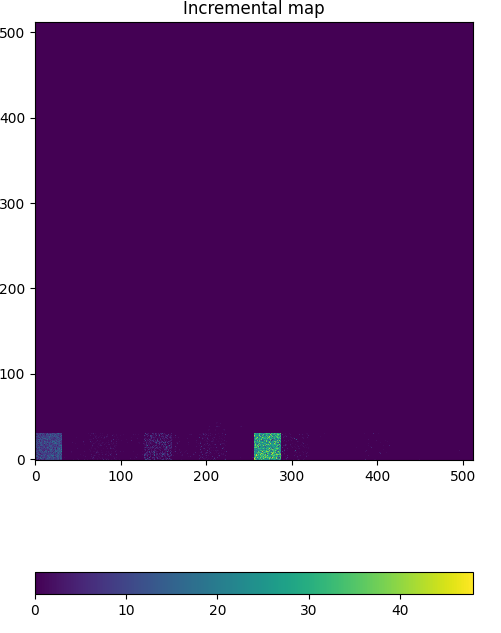
\includegraphics[width=.8\linewidth]{figures/charaterization/ARCADIA/Fe55_5min30s.png} \\
                \centering Fe$^{55}$
                
            \column{0.5\textwidth}    
                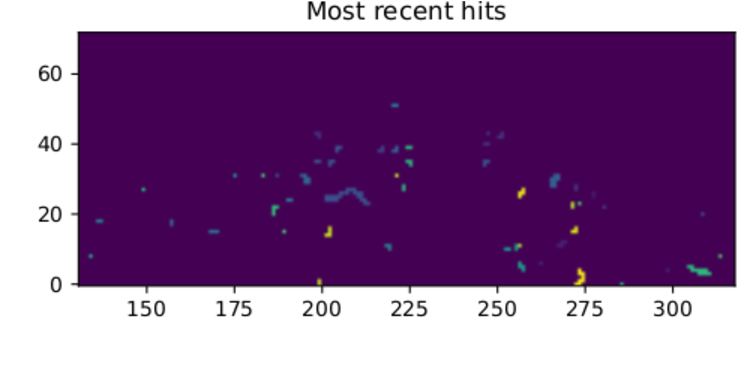
\includegraphics[width=1.\linewidth]{figures/charaterization/ARCADIA/Sr90_2min.pdf}\\
                \centering Sr$^{90}$
        \end{columns}
    \end{frame}